\documentclass[12pt,a4paper]{article}

\usepackage[slovak]{babel}
\usepackage[utf8]{inputenc}
\usepackage[T1]{fontenc}

\usepackage{float}
\usepackage{listings}
\usepackage{graphicx}
\usepackage{tabularx} 

\usepackage{hyperref} 

\usepackage{amsmath} 

\lstset{
language=sh
,breaklines=true
,basicstyle=\ttfamily
, showstringspaces=false}

\author{Peter Csiba}
\textwidth 6.5in
\oddsidemargin 0.0in
\evensidemargin 0.0in

\title{Pánko Herkules vs. Motač Hydra}
\date{12-04-2014}
\author{Peter Csiba, petherz@gmail.com}

\begin{document}
\maketitle

\section*{Abstrakt}
Začalo sa to nevinne. Trošku božia Hera, sestra a manželka Bleskofúzora nahnevalkala nášho Pánka Herkulesa. Ten vo svojom amoku zabil svoju fajnú manželku a šesť synov. "Pipkoš", povedal si Herkules, "Odteraz si budem už len motkať". Následne mu kráľ Eurystheus naložil 12 úloh, a ak ich splní, tak bude zase Pánkom uznaným samotným Bleskofúzorom. 

Druhou úlohou bolo zabiť Motač Hydru. Hydra je zakorenená strom, ktorá má listy=hlavy. Po odseknutí ľubovoľnej hlavy vyrastú nové dva pod-stromy z jej krku=nelistového vrcholu. Takže jak Herkules sečká, tak Hydre rastenkajú hlavy. Vie Herkules zabiť Hydru? Dokážte alebo vyvráťte. Budeme prezentovať dve riešenia. Jedným je brute-force Herkulesove a druhé pochill Goodsteinove z roku 1944. 

\begin{figure}[H]
\centering
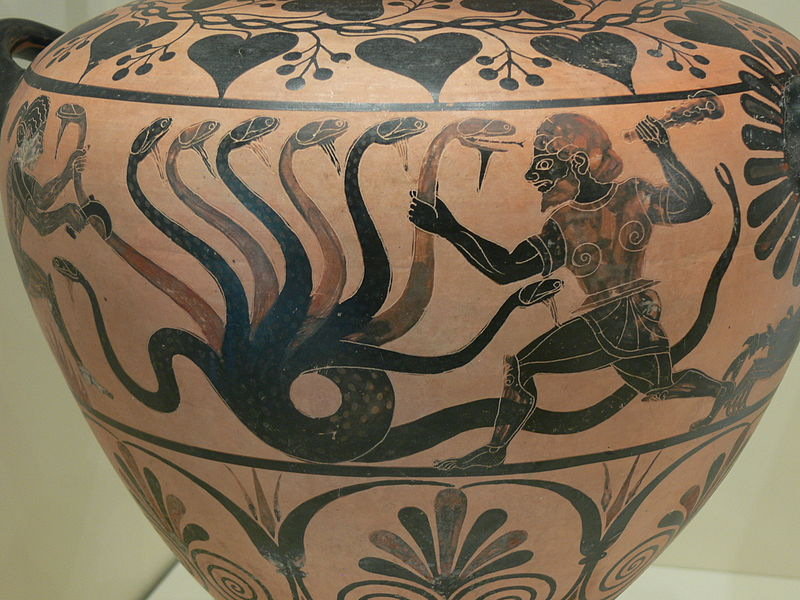
\includegraphics[width=0.6\textwidth]{hydra.png}
\end{figure} 

\section*{Prednáška}

\subsection*{Intro} 

Povedali mi, že dostanem bandu ospalých ľudí a mám pre nich urobiť zaujímavú matematickú prednášku. Ja som si povedal "Pipkoš, challenge accepted". Každá matematická prednáška začina definíciou nášho problému. 

\subsubsection*{Ako rastie Hydra.}
Kto vie ako to v skutočnosti je, nech mlčí o tejto skutočnosti alebo nech ide vedľa :P
You can cut off a head that is connected directly to the root. In that case, nothing grows back. In all other cases, you grow new heads as follows:
\begin{quote}
  \begin{enumerate} 
    \item Let $x$ be the vertex where the head you just cut off was attached to the hydra.
    \item Go down one edge from $x$, let $y$ be the new vertex.
    \item Grow two new copies of the entire subtree you just came from. (We will call this the growth rule.)
  \end{enumerate} 
\end{quote} 

\begin{itemize} 
\item Hlasovanie áno / nevieme / nie. Počas prednášky vás budem presvedčovať o jednej z možností, neverte mi a posudzujte podľa seba. Pamätáme si výsledky hlasovania. 
\end{itemize}

\subsubsection*{Minihra.} 
\begin{itemize}
\item Každá zaujimavá prednáška je dynamická. 
\item Vyberte najmladšieho účastníka, zatiaľ spustíme applet.
\item Najmladší bude Herkules - dostane meč. Ostatní budú hlavy Hydry ako na applete. Spojenia budú realizované rukami. Hlavy nech odstrašujú. \uv{Nech sa pánko Herkules má čoho báť!}.  
\item Herkules seká a Hydra rastie ako na applete. Ostatní mu môžu radiť. 
\item Keď dojdú ľudia, skončí sa intro. 
\item Niekto k notebooku a hrať na applete - ostatní mu radia. 
\end{itemize} 

\subsection*{Vie Herkules vždy vyhrať?}
\begin{itemize}
\item Hlasovanie áno / nevieme / nie. 
\item Ako to v skutočnosti bolo - animácia padajúcej tabule = kameňa na Hydru. Vynásobil nulou. Ak sa vtip ujal, tak ten s $\partial x$, konštantou a $e^x$. 
\end{itemize} 

\subsubsection*{Podobné hry}
\begin{quote}
Kuna rada skáče po prirodzených číslach. Avšak neskáče hocijako, robí len nasledovné skoky: Z čísla $n$ sa vie dostať na číslo $2n$ a naopak. Z čísla $n$ sa vie taktiež dostať na číslo $3n + 1$ alebo naopak. Vie sa z každého prirodzeného čísla nejakou postupnosťou skokov dostať na číslo 1? --  KMS 2007/2008 leto. 
\end{quote} 

\subsubsection*{Collatz conjecture}
\begin{equation}
f(n) = \begin{cases} n/2 &\text{if } n \equiv 0 \pmod{2}\\ 3n+1 & \text{if } n\equiv 1 \pmod{2} .\end{cases}
\end{equation} 
\begin{figure}[H]
\centering
\caption{Každá zaujimavá prednáška má v sebe fraktál.} 
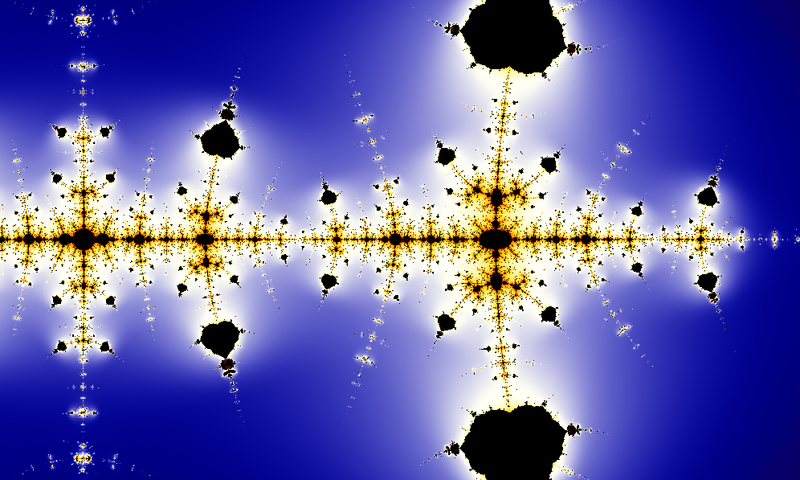
\includegraphics[width=0.6\textwidth]{collatz.png}
\end{figure} 

\subsubsection*{Zbraň matematika - all you can porovnanie} 
\begin{itemize}
\item Pravdou je, že až na konečne veľa prípadov overených počítačom (to je tá informatická zložka), Herkules vždy spapká, preto musel použiť násobenie nulou. 
\item Hlasovanie áno / nevieme / nie. 
\item Ako by ste to dokazovali? 
\item Majme dve hydry, podľa čoho by ste ich porovnali? Predstavte si, že namiesto Pánka Herkulesa, ktorý na zmotanie Motač Hydry použil násobenie nulou, ste matematik, ktorého jediná zbraň je porovnanie. Ak budeme vedieť porovnať každé dve hydry a ukážeme, že to rastie, tak sme vyhrali. Vlastne spapkali.  
\end{itemize} 

\subsubsection*{Pohaluzíme nejaké porovnania.}
\begin{itemize} 
\item počet hláv
\item počet, hĺbka
\item Hlasovanie áno / nevieme / nie. 
\item základná rekurzia 
\item zátvorkovacie výrazy
\item Hlasovanie áno / nevieme / nie. 
\end{itemize} 

\subsubsection*{Ordinálne čísla}
Každá zaujimavá prednáška má svoj WTF moment. 
\begin{figure}[H]
\centering
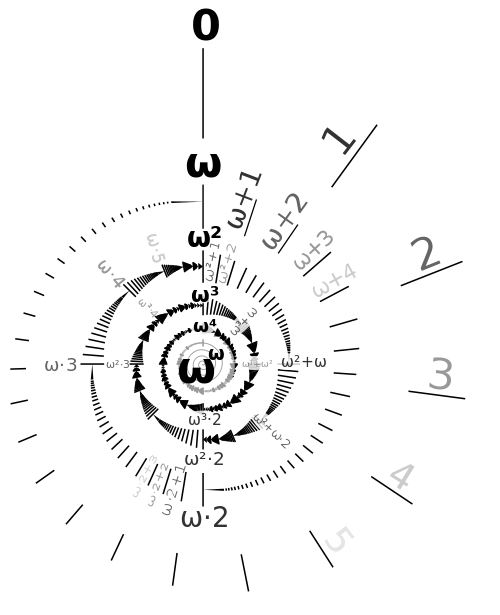
\includegraphics[width=0.8\textwidth]{ordinals.png}
\end{figure} 

\begin{samepage} 
\paragraph{Priklad.} 
Každým sekaním sa zníži exponent. Konkrétne: 
\begin{equation}
w^{w^2 + w^1} + w^2 \rightarrow w^{w^2 + 3} + w^2  \rightarrow 3w^{w^2 + 2} + w^2
\end{equation}
\begin{figure}[H]
\centering
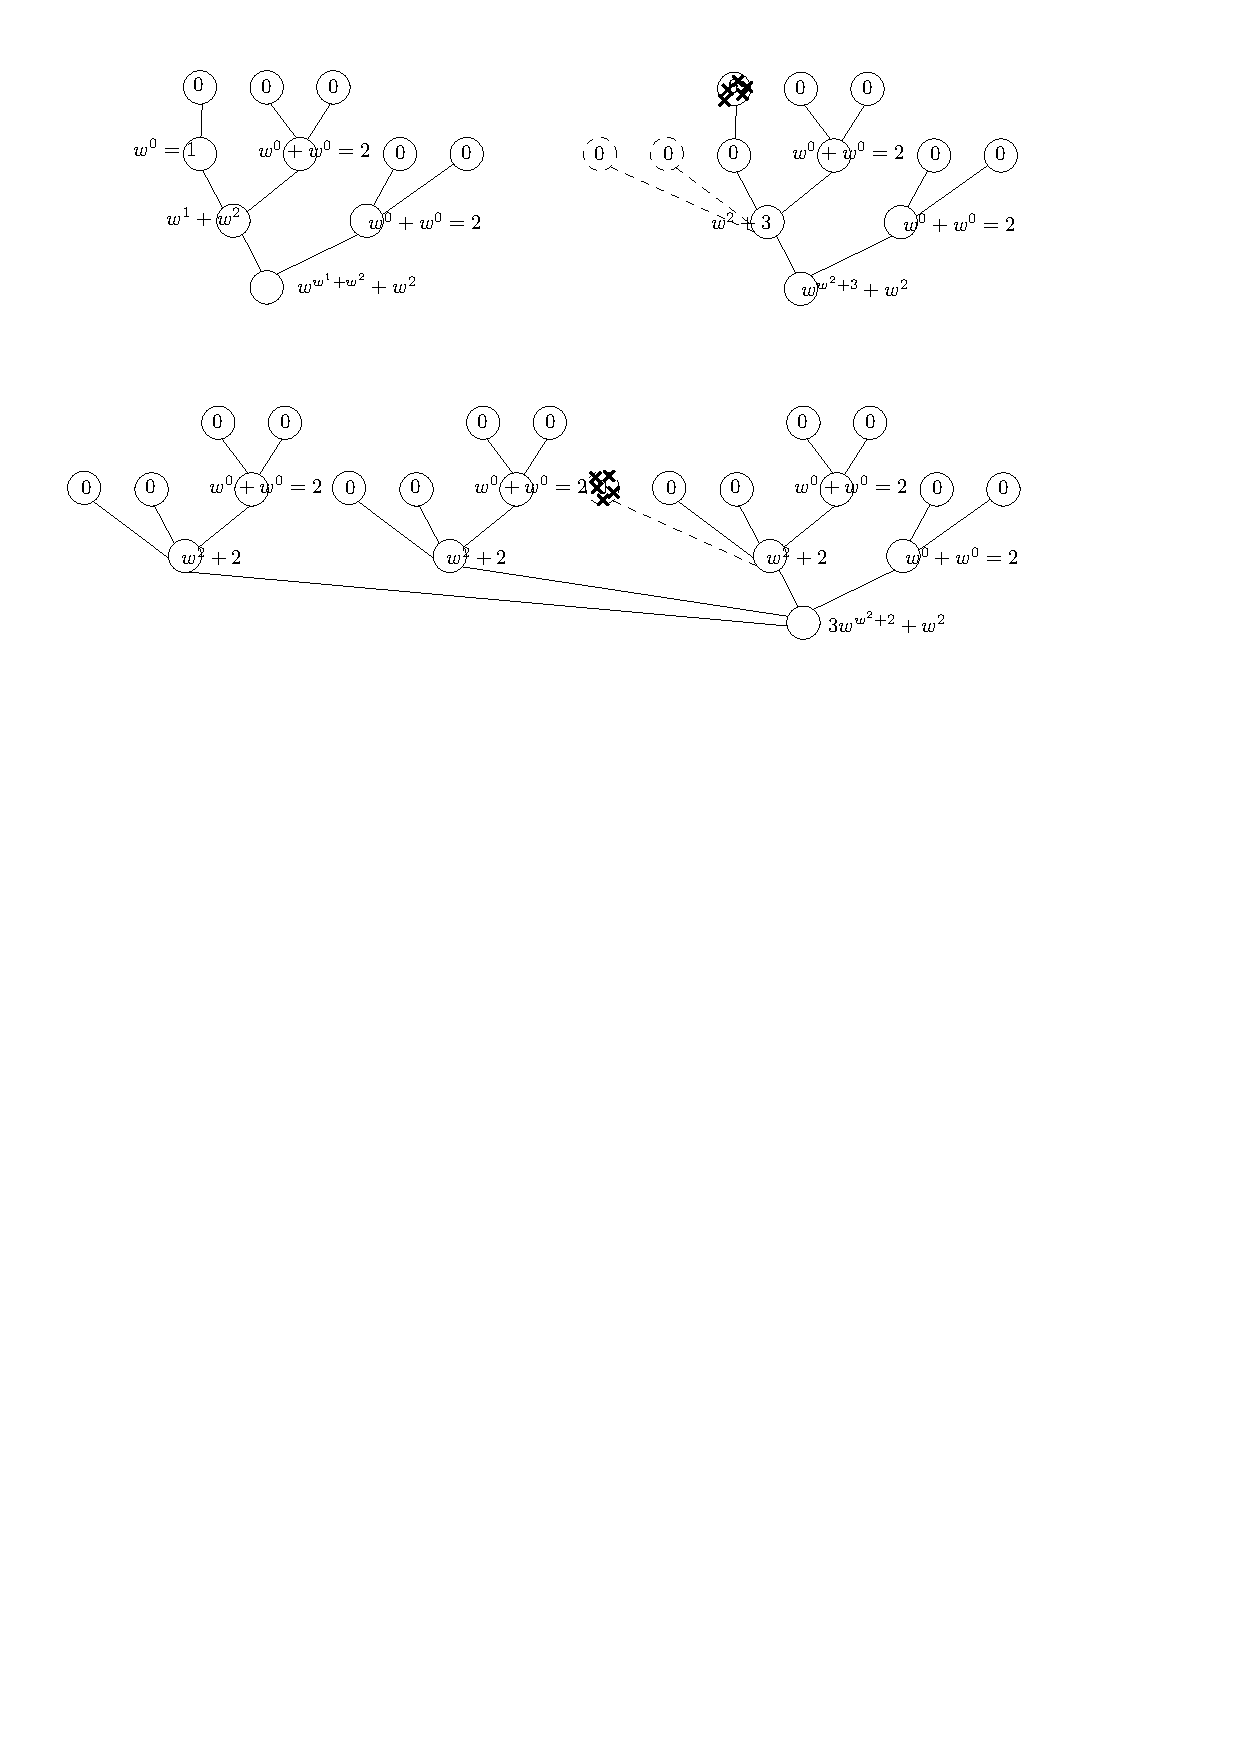
\includegraphics[width=0.8\textwidth]{priklad.pdf}
\end{figure} 
\end{samepage} 

\subsection*{Zovšeobecnenie - area of effect} 

\begin{itemize}
\item Čo keď môže hydre narásť ľubovoľný počet hláv? 
Let's now change the growth rule as follows:
\begin{quote} 
If this is turn $N$ of the game, grow $N$ new copies of the entire subtree you just came from.
That is, the longer you play, the faster the hydra grows.
\end{quote} 
Oops, but you still cannot lose the game. Regardless of how you play, the hydra is still guaranteed to die in finitely many steps.

\item Here's the most awesome version of the growth rule:
\begin{quote} 
Pick any positive integer $N$. Go ahead, make it as large as you wish. You can even pick a different $N$ each time, and make each choice greater than the previous one.
Grow $N$ new copies of the entire subtree you just came from.
\end{quote} 
Guess what? You still cannot lose. Each possible game still has to be finite.

\item Čo keď môže mať "pipkoš" krky?  
  \begin{itemize} 
    \item When a normal neck segment () is cut off, the grandfather node of the severed head, if any, can afterward grow back as many copies as the hydra wishes of the entire subtree from which the head was cut off (i.e., the father node of the severed head and all its descendants).
    \item When a dire neck segment () is cut off, the father node of the severed head can afterward grow back a copy of the entire subtree back from and including the last normal (i.e., non-dire) segment in its ancestors, recursively as deep as the hydra wishes.
  \end{itemize}


\end{itemize} 

\subsection*{Záver} 
\begin{itemize}
\item Predsudky a nepodložené názory iných sú porazené atómovou bombou matematiky a faktov - odteraz keď budete čítať články, pozrite si referencie. 
\item Vidíte. Myslieť hlavou sa oplatí. Kým na Herkulesovu bruteforce metódu by ste riadne napotili, keď ste matematik tak vám stačí random klikať a aura porovnania zmotká za vás. 
\item Hlasovanie áno / nevieme / nie. 
\end{itemize} 

\subsection*{Bonus} 

\begin{figure}[H]
\centering
\caption{Po pár hodinách automatického sekania.} 
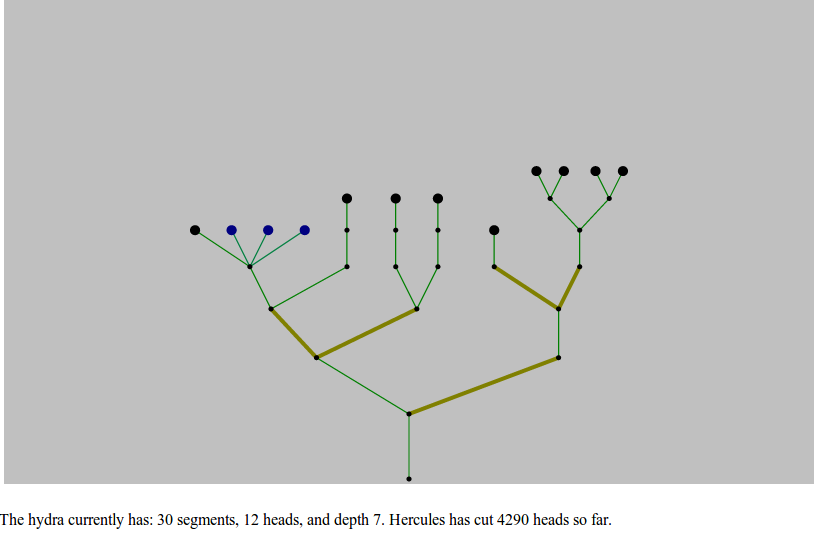
\includegraphics[width=0.8\textwidth]{herkules_secka.png}
\end{figure} 

\begin{figure}[H]
\centering
\caption{Po pár dňoch automatického sekania.} 
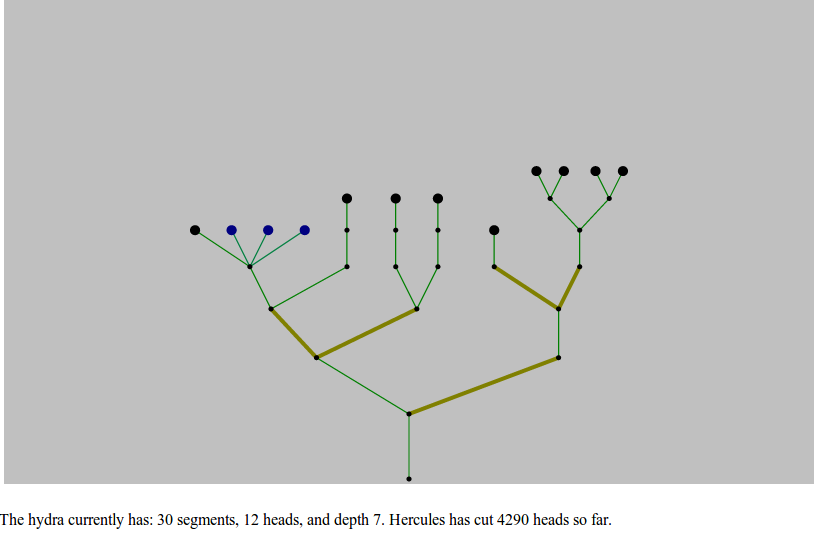
\includegraphics[width=0.8\textwidth]{herkules_secka.png}
\end{figure} 

\section*{Zdroje} 
\begin{itemize} 
\item \href{http://www.quora.com/Mathematics/What-are-some-of-the-most-counterintuitive-mathematical-results/answer/Michal-Fori\%C5\%A1ek?ref=fb}{Pôvodná inšpirácia}
\item \href{http://en.wikipedia.org/wiki/Lernaean_Hydra}{Abstrakt = Príbeh}  
\item \href{http://en.wikipedia.org/wiki/Ordinal_number}{Ordinálne čísla}
\item \href{http://en.wikipedia.org/wiki/Goodstein's_theorem}{Dôkaz}
\item \href{http://www.madore.org/~david/math/hydra.xhtml}{Applet 1 (by David A. Madore)} 
\item \href{http://math.andrej.com/wp-content/uploads/2008/02/Hydra/hydraApplet.html}{Applet 2 (by Andrej Bauer)} Idealne stiahnut .jar a prikaz: 
\begin{lstlisting}
java -cp hydra.jar hydra.HydraWindow
\end{lstlisting}
\end{itemize} 

\end{document}

